\documentclass[12pt]{article}
\usepackage[spanish]{babel }
\usepackage{graphicx}
\usepackage{float}
\usepackage{hyperref}
\usepackage{times}
%opening
\title{\textbf{\textit{\underline{¿Inundación o Sequía?}}}}

\begin{document}
	
\begin{titlepage}
	\centering
	\vspace*{1cm}
	\begin{figure}
		\centering
		
\includegraphics[width=0.3\linewidth]{./Report/images/logo}
		\label{fig:logo}
	\end{figure}
	
	\large{\textbf{Universidad de La Habana}\\
	Facultad de Matemática y Computación\\}
	\vspace{3.5cm}
	
	{\rmfamily\selectfont\Huge{Adentrémonos en el mundo de la sequía.}} 
	\vspace{1.5cm}
	
	\Large
	\vspace{2 cm}
	\normalsize{\textbf{Autores:}\\
		Jennifer de la Caridad Sánchez Santana\\
		Angélica María Martínez Céspedez\\
		Guillermo Ferriol Ravelo\\
		Diego Puentes Fernández\\}
	\vfill
	
	\large
	\today
\end{titlepage}

	
	\begin{center}
		\textbf{\textit{\underline{{\fontsize{60}{24}\selectfont ¿Sequía?:}}}}
	\end{center}
	
	
	Imagina un mundo donde la tierra se agrieta bajo el sol implacable, donde los ríos se convierten en hilos de agua apenas perceptibles, y donde la sed se convierte en una compañera constante. Este es el mundo de la sequía, un fenómeno que va más allá de la simple escasez de agua, para sumergir a comunidades enteras en una lucha desesperada por la supervivencia.
    \par\vspace{4mm}
	\begin{figure}[H]
		\centering
		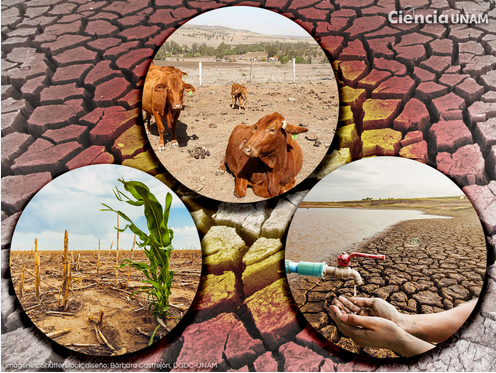
\includegraphics[width=0.7\linewidth]{./Report/images/4.png}
		\label{fig:ian}
	\end{figure}
	\par\vspace{4mm}
	Las sequías son periodos prolongados de tiempo seco causados por la falta de lluvia, lo que produce escasez de agua. Este fenómeno desencadena una serie de impactos devastadores en la vida de las personas y en los ecosistemas. La sequía afecta a todas las regiones del planeta, en menor o mayor medida, y es una consecuencia del cambio climático, lo que hace que este fenómeno nos visite cada vez más seguido y por más tiempo y por supuesto, nuestra paradisíaca isla de Cuba no es ajena a sus efectos.
	
	\section{Causas de las sequías}
	Algunas de las principales causas de las sequías son :
    \begin{itemize}
		\item Cambio climático: El calentamiento global debido a la acumulación de gases de efecto invernadero en la atmósfera está alterando los patrones climáticos y aumentando la frecuencia e intensidad de eventos climáticos extremos, incluidas las sequías y el derretimiento de glaciares, por mencionar solo algunos de sus efectos.

		\item Deficiencias en las precipitaciones: La falta de lluvias o nevadas suficientes durante la temporada de crecimiento puede llevar a una sequía en la región afectada.

		\item Agotamiento de fuentes de agua: El uso excesivo de recursos hídricos, como aguas subterráneas y ríos, para el riego agrícola, puede llevar al agotamiento de las fuentes de agua locales y a la sequía.

		\item Deforestación: Aunque no se vea la relación a simple vista, la tala masiva de bosques reduce la capacidad de retención de agua del suelo y afecta el ciclo hidrológico, lo que puede contribuir a la sequía. Esto es particularmente relevante en América del Sur, donde se siente cada vez más la reducción del Amazonas, principal reserva de bosques del mundo.

		\item Prácticas agrícolas inadecuadas: El uso ineficiente del agua en la agricultura, como el riego inadecuado o la falta de técnicas de conservación de agua, puede aumentar la vulnerabilidad de una región a la sequía. Al día de hoy, las nuevas tecnologías y métodos distintos de riego promueven un uso más racional del agua.

		\item Urbanización y crecimiento de la población: El aumento de la población y la expansión urbana pueden aumentar la demanda de agua, presionando aún más los recursos hídricos disponibles para la agricultura. Al mismo tiempo, la contaminación de fuentes de agua puede afectar su calidad y disponibilidad para el riego y el consumo humano.

		\item Sobrepastoreo y degradación del suelo: Prácticas agrícolas y ganaderas mal gestionadas pueden dañar el suelo y reducir su capacidad para retener agua, lo que puede agravar la sequía.
	\end{itemize}
	
	\section{Sequía en Cuba}
    \begin{figure}
		\centering
		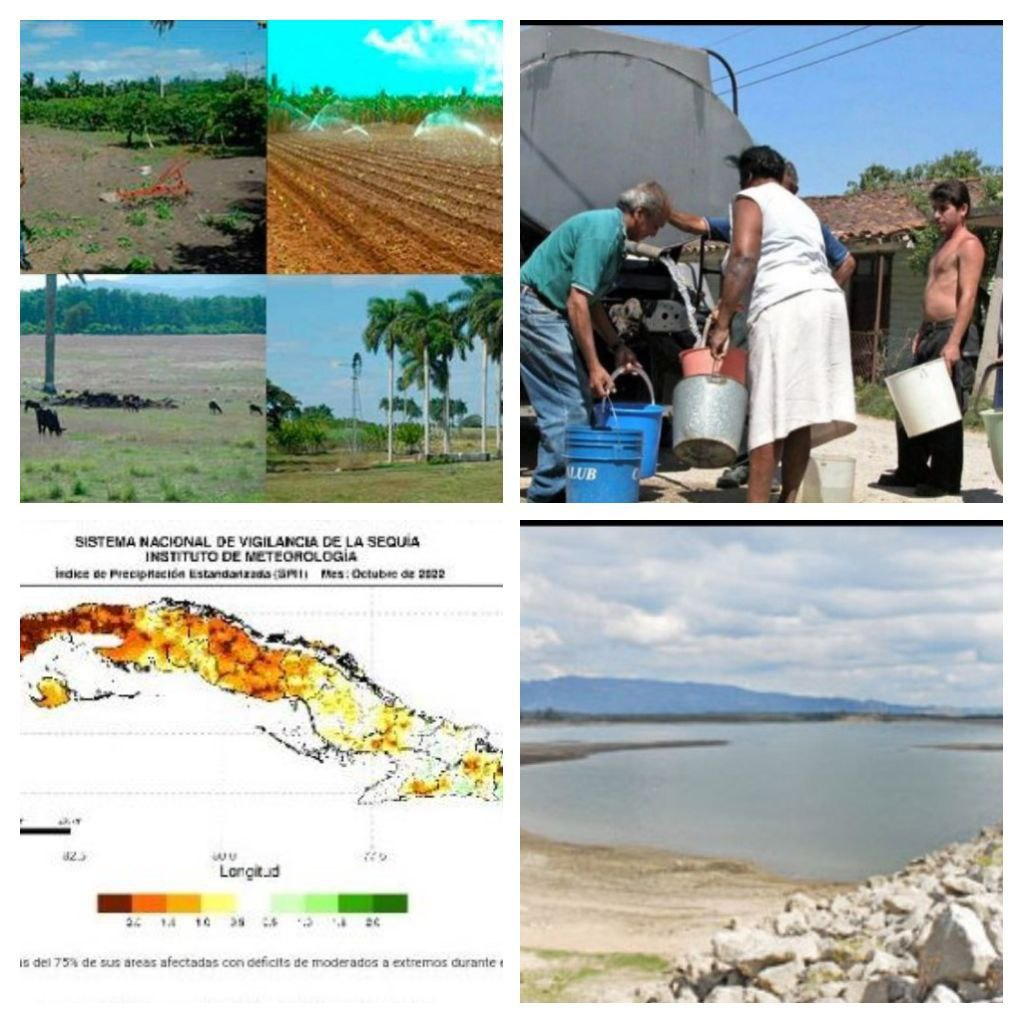
\includegraphics[width=0.7\linewidth]{./Report/images/9.jpg}
	\end{figure}

	\newpage
    Dada su posición geográfica, el archipiélago cubano está situado en una zona climática donde normalmente llueve cada año en el verano. Durante el invierno, los frentes fríos pueden venir acompañados de abundantes precipitaciones, a lo que se añaden las tormentas y los ciclones pluviosos.
    \par\vspace{4mm}
    Sin embargo, con el incremento de la población, ocurre el aumento exponencial del consumo de agua, así como la contaminación de algunas fuentes. Esto en Cuba contribuye a que la disponibilidad de agua por habitantes sea crítica. Por eso, durante varios meses o años las precipitaciones son escasas y se mantienen por debajo de los promedios históricos, y no ocurren huracanes o tormentas pluviales,siendo ahí cuando se presentá la sequía.
    \par\vspace{4mm}
    En Cuba tenemos reservas de agua potable en los ríos, en las lagunas, en los pantanos y en el subsuelo. Pero esas reservas se alimentan de las lluvias de verano y de las que acompañan los huracanes, cuya escasez o ausencia puede conducir a la sequía.
    \begin{figure}
		\centering
		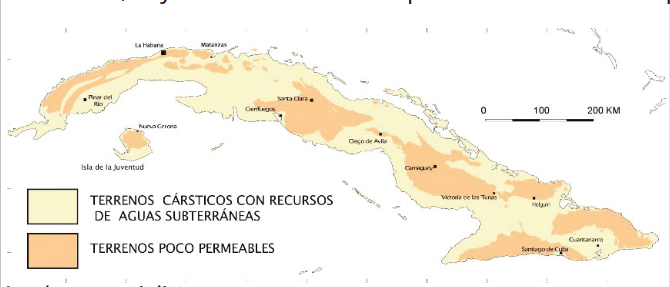
\includegraphics[width=0.7\linewidth]{./Report/images/10.png}
		\caption{Mapa de Cuba según la ubicación de las reservas acuíferas}
	\end{figure}
	\newpage
    El déficit de precipitaciones y sus acumulados se prolongan de mes en mes, de año en año, hasta que inevitablemente comenzamos a padecer de sus efectos, siendo los principales años en estas últimas tres décadas los que más lo sufrieron:  2000,2004, 2009, 2015 y 2021, todos con acumulados anuales por debajo de los 12000 mm. En 2004 ocurrió la más severa sequía de los últimos 100 años. Especialmente en esta fecha, ya se venía acumulando el déficit; cada vez llovía menos. Siendo en ese mismo año, apenas en dos de sus meses que tuvieron acumulados por encima de la media.
	\par\vspace{2pt}
	\begin{figure}
		\centering
		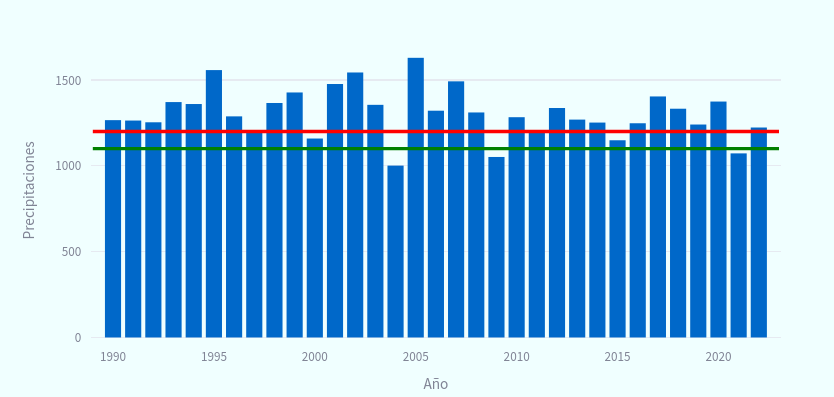
\includegraphics[width=0.8\linewidth]{./Report/images/1.png}
		\caption{Gráfico de cómo se comportaron los niveles de precipitación anuales.}
	\end{figure}
	\begin{figure}
		\centering
		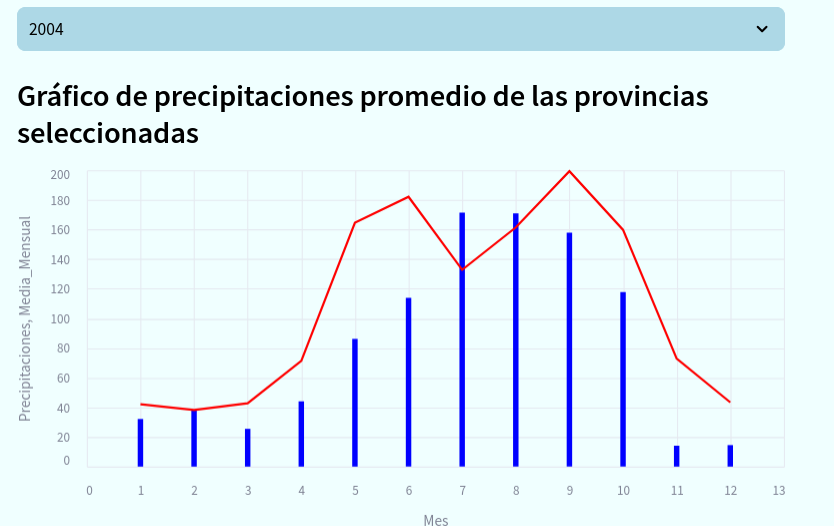
\includegraphics[width=0.7\linewidth]{./Report/images/2.png}
		\caption{Gráfico de cómo se comportaron los niveles de precipitación en el año 2004.}
	\end{figure}
	\newpage
	\section{A quienes afecta la sequía}
	
    En los últimos años, los incrementos de los episodios de sequía han traído consecuencias para los seres humanos, la agricultura y la sociedad, entre las que encontramos:
    \par\vspace{4mm}
    1. Agricultores y ganaderos: La falta de lluvias reduce la disponibilidad de agua para regar cultivos y para el consumo de los animales, lo que puede llevar a la pérdida de cosechas y a la escasez de forraje para el ganado.
    \par\vspace{4mm}
    2. Comunidades rurales: Aquellas que dependen de fuentes de agua locales para el consumo humano y actividades agrícolas pueden enfrentar escasez de agua potable y riego, lo que afecta la salud, la producción de alimentos y la economía local.
    \par\vspace{4mm}
    3. Consumidores: La sequía puede llevar a la escasez de alimentos y a un aumento en los precios de los productos agrícolas, lo que impacta en la seguridad alimentaria y en los bolsillos de las personas.
    \par\vspace{4mm}
    4. Industrias: La falta de agua puede afectar a sectores como la producción de energía, la manufactura, la minería y el turismo, entre otros.
    \par\vspace{4mm}
    5. Medio ambiente: La sequía puede provocar la pérdida de hábitats naturales, la disminución de recursos hídricos y afectar a la flora y fauna locales, así como la desertificación y la erosión.
    \par\vspace{4mm}
    6. Salud pública: La escasez de agua puede llevar a problemas de higiene, saneamiento y salud, así como a la propagación de enfermedades relacionadas con el agua.
    \par\vspace{4mm}
    La sequía es inevitable, así que el único modo de reducir sus efectos negativos es prepararnos con anticipación, tomando medidas inteligentes mucho antes de que se presente. Sobre todo, cuando sabemos que a consecuencia del Cambio Climático hay una tendencia a la reducción de las precipitaciones y un recrudecimiento de los períodos de sequía, que se presentan cada vez con mayor frecuencia. A continuacion se encuentran algunos ejemplos de medidas que se pueden tomar.
	\begin{figure}[H]
		\centering
		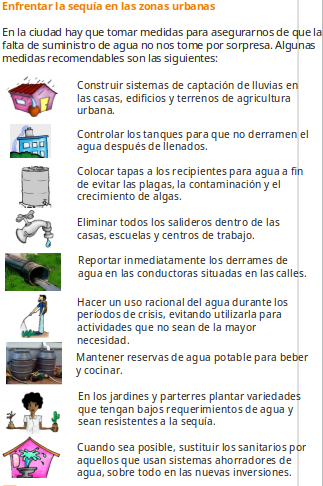
\includegraphics[width=0.8\linewidth]{./Report/images/6}
	\end{figure}
	\begin{figure}[H]
		\centering
		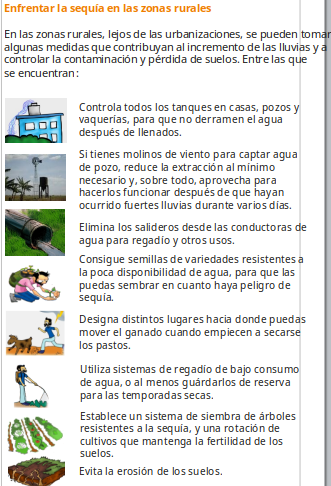
\includegraphics[width=0.8\linewidth]{./Report/images/7}
	\end{figure}
	
	
	\newpage
	\begin{thebibliography}{8}
		\bibitem{webpage1} 
		\url{https://www.droughtmanagement.info/literature/UNW-DPC_NDMP_Country_Report_Cuba_2013.pdf}
		
		\bibitem{webpage2}
		\url{https://agriplasticscommunity.com/es/impacto-de-la-sequia-en-la-agricultura-consecuencias-y-soluciones/}
		
		\bibitem{webpage3}
		\url{https://rotoplas.com.ar/agroindustria/como-afecta-la-sequia-a-los-cultivos-y-como-evitarlo/}
		
		\bibitem{webpage4}
		\url{http://www.redciencia.cu/uploads/protegete/2018_Folleto9_sequia.pdf}
		
	\end{thebibliography}
	
	
\end{document}